\newpage

\chapter{lecture 10/03/2025}

\section{Tumor Size over Time}

Let's consider an example case of a tumor growth. Let's assume that $X(t)$ is the size of a tumor at time $t$.

The differential equation that describes the growth of the tumor is:

$$
X(t + dt) = X(t) + \Phi X(t) - M X(t)
$$

where $\Phi$\ is the growth rate and $M$ is the decay rate.

We can rewrite the equation as:

$$
\dfrac{X(t + dt) - X(t)}{dt} = X(t) \dfrac{(\Phi - M)}{dt}
$$

Let's rewrite \Phi\ and M as:

$$
\begin{array}{l}
\Phi = b dt + \cancel{O(dt^2)} \\
M = m dt + \cancel{O(dt^2)}
\end{array} \quad \text{(We neglect the higher order terms)}
$$

We obtain the following differential equation:

$$
\dfrac{X(t + dt) - X(t)}{dt} = X(t) (b - m) \quad \Rightarrow \quad \dfrac{dX}{dt} = X(b - m)
$$

Often we have a starting condition $X(0) = X_0$. Defining $a = b - m$, the sistem becomes:

$$
\begin{cases}
    \dfrac{dX}{dt} = aX \\
    X(0) = X_0
\end{cases}
$$

Since makes no sense to have a negative time or tumor size, we have the constraints:

$$
\begin{cases}
    t \in \mathbb{R}^+ \cup \{0\} \\
    X \in \mathbb{R}^+ \cup \{0\}
\end{cases}
$$

The solution is given by:

$$
X(t) = X_0 e^{at}
$$

$$
X(t + dt) = X(t) + b dt X - mdt X - \theta dt X
$$

$$
\begin{cases}
\dot X = (a - \theta) X
X(0) = X_0
\end{cases}
$$

dunque la soluzione è:

$$
X(t) = X_0 e^{(a - \theta)t}
$$

In questo caso, per $a > \theta$, il tumore cresce esponenzialmente, mentre per $a < \theta$, il tumore decresce esponenzialmente.

Nella realtà però il valore \theta \ non è costante nel tempo, ma varia nel tempo. In tal caso il sistema diventa:

$$
\begin{cases}
\dot X = (a - \theta(t)) X \\
X(0) = X_0
\end{cases}
$$

e la soluzione è:

$$
X(t) = X_0 e^{\int_0^t (a - \theta(s)) ds}
$$


Più in generale, un sistema del tipo:

$$
z(y) = e^{G(y)} b
$$

si ha

$$
\frac{dz}{dy} = \frac{d}{dy} e^{G(y)} b = e^{G(y)} b \frac{dG}{dy} = G'(y)z(y)
$$

Esempio:

$$
\begin{cases}
    Z'(t) = \sin(t) Z(t) \\
    Z(0) = Z_0
\end{cases}
$$

Si ha:

$$
\begin{cases}
Z(t) = e^{-\cos(t)} B \\
Z_0 = e^{-1} B
\end{cases}
\quad \Rightarrow \quad
Z(t) = e^{1-\cos(t)} z_0
$$

\newpage

\section{Stabily and Eq. Points}

\subsection{Equilibrium Points}

Given the system:

$$
\begin{cases}
    \dot x = f(x) \\
    x \in \mathbb{R}^n
\end{cases}
$$

An equilibrium point is a point $x^*$ such that $f(x^*) = 0$.

\begin{tipsblock}[Eq. points]
A system can have multiple equilibrium points.
\end{tipsblock}

We have three kinds of equilibrium:

\begin{itemize}
    \item \textbf{Stable equilibrium}: if the system is in the neighborhood of the equilibrium point, it will remain there.
    \item \textbf{Neutral equilibrium}: if the system is in the neighborhood of the equilibrium point, it will remain there, but it will not return to it.
    \item \textbf{Unstable equilibrium}: if the system is in the neighborhood of the equilibrium point, it will move away from it.
\end{itemize}

\begin{figure}[H]
    \centering
    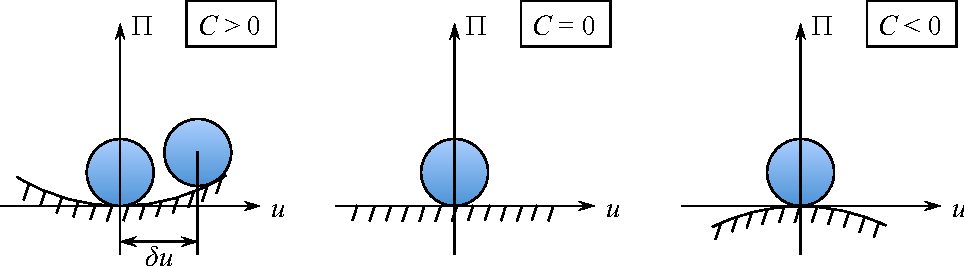
\includegraphics[width=0.65\textwidth]{assets/eq_points.png}
    \caption{Stable, Natural and Unstable Equilibrium Points \cite{stability}}
\end{figure}

\subsection{Stability}

We say that a system is \textbf{\textit{Globally Asymptotically Stable}} (or \textit{Globally Attractive}) if it is stable and if it converges to the equilibrium point from any initial condition.

\newpage
\section{Local Analysis Near the Equilibrium Point}

In this section, we study the system in the neighborhood of the equilibrium point. Let the initial condition be a small perturbation around the equilibrium:

$$
X(0) = X_e + \varepsilon.
$$

We introduce a deviation function $U(t)$ defined by

$$
X(t) = X_e + U(t),
$$

with the initial condition

$$
U(0) = \varepsilon.
$$

Thus, the evolution of the perturbation is governed by

$$
\begin{cases}
\dot U = f(X_e + U), \\
U(0) = \varepsilon.
\end{cases}
$$

Assume that the dynamics of the system are given by

$$
\dot X = X(b(X) - m(X)).
$$

Then the perturbed system becomes

$$
\dot U = (b(X_e + U) - m(X_e + U))(X_e + U).
$$

Expanding $b(X_e + U)$ and $m(X_e + U)$ in a Taylor series around $X_e$, we have:

$$
b(X_e + U) \approx b(X_e) + b'(X_e)U,
$$
$$
m(X_e + U) \approx m(X_e) + m'(X_e)U.
$$

Substituting these into the equation for $\dot U$, we get:

$$
\begin{array}{rl}
\dot U & = \bigl[b(X_e) + b'(X_e)U\bigr] - \bigl[m(X_e) + m'(X_e)U\bigr](X_e + U) \\
      & = \bigl[b(X_e) + b'(X_e)U\bigr] - \bigl[m(X_e)X_e + m(X_e)U + m'(X_e)X_eU + m'(X_e)U^2\bigr].
\end{array}
$$

Since the equilibrium condition implies that

$$
(b(X_e) - m(X_e))X_e = 0,
$$

the above expression simplifies (neglecting the higher-order term $m'(X_e)U^2$) to:

$$
\dot U \approx \left[b'(X_e) - m(X_e) - m'(X_e)X_e\right] U.
$$

Under the assumption that $b'(X_e)$ is negative, we can express this as

$$
\dot U \approx -X_e\Bigl(|b'(X_e)| + m'(X_e)\Bigr)U.
$$

The solution of this linearized differential equation is given by:

$$
U(t) = U(0)\,e^{-X_e (|b'(X_e)| + m'(X_e))t}.
$$

Hence, we identify the decay rate (or the inverse of the characteristic time constant) as

$$
X_e\Bigl(|b'(X_e)| + m'(X_e)\Bigr),
$$

and the characteristic time $\tau$ is:

$$
\tau = \frac{1}{X_e \left(|b'(X_e)| + m'(X_e)\right)}.
$$

This time constant represents the rate at which perturbations decay in the vicinity of the equilibrium point.


\newpage

$$
X(t) = X_e + U(t) \Rightarrow \dot U = f(X_e + U) = \underbrace{f(X_e)}_{=\ 0} + f'(X_e)U + O(U^2)
$$

$$
\dot U = f'(X_e)U \Rightarrow U(t) = U(0) e^{f'(X_e)t}
$$

So we have:
$$
\begin{cases}
f'(X_e) < 0 \quad \Rightarrow \quad X_e \text{ is Locally Asintotically stable } \\
f'(X_e) > 0 \quad \Rightarrow \quad X_e \text{ is Unstable }
\end{cases}
$$

\vspace{2em}

\section{Non-scalar Systems}

Consider the system:

$$
\begin{cases}
    \dot x = f(x) \\
    x \in \mathcal{f} \subseteq \mathbb{R}^n
\end{cases}
$$

As in the scalar case, we can linearize the system around the equilibrium point $x_e$:

$$
f(X_e) = 0
$$

$$
X = X_e + U, \quad \quad |U| \ll 1
$$

We have to consider the Jacobian matrix of $f$:

\dots

\newpage

\section{Exponential of a Matrix}

Let's consider a linear system of the form:

$$
\dot x = Ax
$$

where $A \in \mathbb{R}^{n \times n}$ is a matrix. The solution of this system is given by:

$$
x(t) = e^{At} x(0)
$$

where $e^{At}$ is the exponential of the matrix $A$.

\begin{definitionblock}[Exponential of a Matrix]
Given a matrix $A \in \mathbb{R}^{n \times n}$, the exponential of $A$ is defined as:

$$
e^A = I + A + \frac{A^2}{2!} + \frac{A^3}{3!} + \dots = \sum_{k=0}^{\infty} \frac{A^k}{k!}
$$

This comes from the Taylor series expansion of the exponential function.
\end{definitionblock}

$$
\dfrac d{dt} e^{At} = \sum_{m = 1}^\infty A^m m \dfrac{t^{m-1}}{m(m-1)!}
= \sum_{k = 0}^\infty A A^k \dfrac{t^k}{k!}
= A e^{At}
$$

$$
\begin{array}{lll}
A & = & H \cdot \text{Diag}(\lambda_1, \lambda_2, \dots, \lambda_n) \cdot H^{-1} \\
A^2 & = & H \cdot \text{Diag}(\lambda_1^2, \lambda_2^2, \dots, \lambda_n^2) \cdot H^{-1} \\
A^m & = & H \cdot \text{Diag}(\lambda_1^m, \lambda_2^m, \dots, \lambda_n^m) \cdot H^{-1}
\end{array}
$$

So we have:

$$
e^{At} = \sum_{m = 0} ^ \infty \dfrac{A^m t^m}{m!} = 
$$

\newpage

An example of a matrix exponential is given by the Newton's law:

$$
m \ddot x = F
$$

Let's consider a more complex case with air resistance $\gamma$:

$$
m \ddot x = - \gamma \dot x - F(x)
$$

We can rewrite this system as:

